La figura representa el sólido del primer octante comprendido entre el plano $y=x$ y el cilindro parabólico $z=9-x^2$. Formule $\iiint_E f\,dV$ en los órdenes $dz\,dy\,dx$ y $dy\,dx\,dz$.

\begingroup
\shorthandoff{>}
\begin{center}
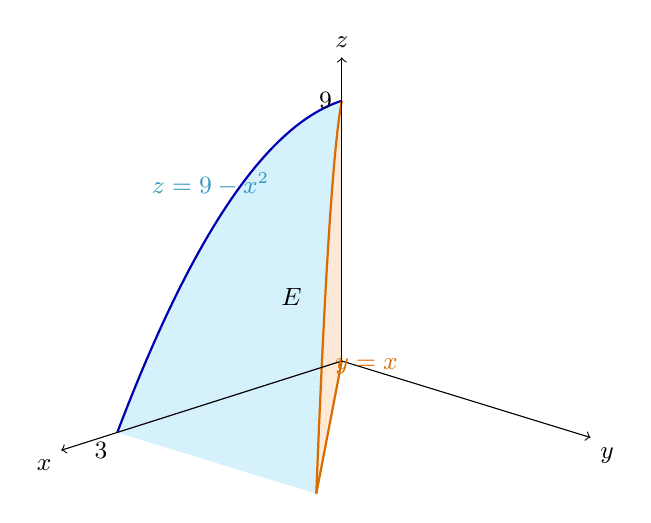
\begin{tikzpicture}[
    x={(-.88cm,-.28cm)},y={(.78cm,-.24cm)},z={(0cm,.34cm)},
    scale=1.08,every node/.style={font=\small}]
    \foreach \i in {0,...,17} {
        \pgfmathsetmacro{\xa}{3*\i/18}
        \pgfmathsetmacro{\xb}{3*(\i+1)/18}
        \fill[blue!11]
            (\xa,0,0) -- (\xb,0,0) -- (\xb,0,{9-\xb*\xb}) --
            (\xa,0,{9-\xa*\xa}) -- cycle;
        \fill[orange!17]
            (\xa,\xa,0) -- (\xb,\xb,0) --
            (\xb,\xb,{9-\xb*\xb}) -- (\xa,\xa,{9-\xa*\xa}) -- cycle;
        \fill[cyan!17]
            (\xa,0,{9-\xa*\xa}) -- (\xa,\xa,{9-\xa*\xa}) --
            (\xb,\xb,{9-\xb*\xb}) -- (\xb,0,{9-\xb*\xb}) -- cycle;
    }
    \draw[blue!70!black,thick]
        plot[domain=0:3,samples=50] (\x,0,{9-\x*\x});
    \draw[orange!85!black,thick]
        plot[domain=0:3,samples=50] (\x,\x,{9-\x*\x});
    \draw[orange!85!black,thick] (0,0,0) -- (3,3,0);
    \draw[gray!65] (0,0,0) -- (3,0,0);
    \draw[gray!65] (0,0,9) -- (0,0,0);
    \draw[->] (0,0,0) -- (3.75,0,0) node[below left] {$x$};
    \draw[->] (0,0,0) -- (0,3.75,0) node[below right] {$y$};
    \draw[->] (0,0,0) -- (0,0,10.5) node[above] {$z$};
    \node[below left] at (3,0,0) {$3$};
    \node[left] at (0,0,9) {$9$};
    \node[cyan!75!black,left] at (1.15,.35,7.3) {$z=9-x^2$};
    \node[orange!85!black,right] at (1.9,1.9,2.7) {$y=x$};
    \node at (1.25,.65,3.7) {$E$};
\end{tikzpicture}
\end{center}
\endgroup
